% ============================================================
%  Final Project Report
%  Course: [Your Course Name / Number]
%  Deadline: May 13, midnight (AoE) — STRICT
% ============================================================
\documentclass[11pt]{article}

% ----- Page layout -----
\usepackage[margin=1in]{geometry}
\usepackage{setspace}           % line-spacing helpers if needed

% ----- Fonts & encoding -----
\usepackage[T1]{fontenc}
\usepackage[utf8]{inputenc}
\usepackage{lmodern}

% ----- Math -----
\usepackage{amsmath, amssymb, amsthm}

% ----- Graphics & figures -----
\usepackage{graphicx}
\usepackage{subcaption}         % side-by-side subfigures
\usepackage{float}              % [H] placement
\usepackage{tikz}               % optional inline diagrams

% ----- Tables -----
\usepackage{booktabs}
\usepackage{multirow}

% ----- Code listings -----
\usepackage{listings}
\usepackage{xcolor}
\lstset{
  basicstyle=\ttfamily\small,
  keywordstyle=\color{blue}\bfseries,
  commentstyle=\color{gray}\itshape,
  stringstyle=\color{teal},
  numbers=left,
  numberstyle=\tiny\color{gray},
  frame=single,
  breaklines=true,
  captionpos=b
}

% ----- Hyperlinks -----
\usepackage{hyperref}
\hypersetup{
  colorlinks=true,
  linkcolor=blue,
  citecolor=blue,
  urlcolor=blue
}

% ----- Bibliography -----
\usepackage{natbib}             % \citep / \citet style; swap for biblatex if preferred

% ----- Miscellaneous -----
\usepackage{microtype}          % better justification
\usepackage{enumitem}           % compact lists
\usepackage{algorithm}
\usepackage{algpseudocode}


\algblockdefx[ParFor]{ParFor}{EndParFor}[1]
  {\textbf{for} #1 \textbf{do in parallel}}
  {\textbf{end for}}

% ============================================================
%  Figure path for model-parallelism charts.
%  Adjust this one line to match your results directory.
% ============================================================
\newcommand{\mpfig}[1]{images/#1} 

% ============================================================
%  Title block
% ============================================================
\title{
  \textbf{MPI Parallelization of MLP Training on MNIST} \\[4pt]
  \large Final Project Report
}

\author{
  Author One\thanks{Equal contribution.} \quad
  Author Two$^*$ \quad
  Author Three \\[2pt]
  \textit{[Course Name \& Number, Institution]}
}

\date{May 2026}

% ============================================================
\begin{document}
\maketitle

% GitHub repo — required by submission guidelines
\begin{center}
  \textbf{GitHub Repository:}
  \href{https://github.com/your-org/your-repo}{\texttt{github.com/your-org/your-repo}} % TODO: replace with final URL
\end{center}

\begin{abstract}
  We study how far MPI-based parallelism can accelerate end-to-end neural-network
  training while preserving training quality under controlled settings. Starting
  from a serial C++17 MLP baseline on MNIST, we implement and compare four MPI
  execution modes: flat data parallelism, two-level hierarchical data
  parallelism, local-SGD with periodic synchronization, and layer-wise model
  parallelism. To keep comparisons fair, all backends use matched model shape,
  optimizer configuration, dataset subsets, and output metrics schema, and are
  launched with one thread per rank for BLAS/OpenMP runtimes. We also apply
  shared engineering optimizations such as memory reuse in hot paths and release
  compiler settings. The main empirical outcome is that communication structure,
  not only rank count, determines realized speedup: local-SGD gives the best raw
  epoch-time scaling at large cluster size, flat DP remains a strong and stable
  baseline, hierarchical DP does not outperform flat DP for the current model
  size, and model parallelism is most sensitive to partition balance and
  communication boundaries.
\end{abstract}

% ============================================================
\section{Hypothesis}
\label{sec:hypothesis}
% ---------------------------------------------------------------
% State the question you want to investigate.
% What did you expect to find, and what did you actually find?
% ---------------------------------------------------------------

We investigate whether communication-aware MPI training strategies can deliver
better time-to-epoch than a standard flat all-reduce baseline while maintaining
comparable optimization behavior on MNIST. Our hypothesis has two parts:
\begin{itemize}[nosep]
  \item communication pattern matters as much as rank count, so methods that
        reduce or amortize global synchronization should scale better at larger
        process counts;
  \item implementation details (memory reuse, consistent launch semantics, and
        stable timing definitions) are necessary to expose the true algorithmic
        differences across backends.
\end{itemize}
The observed results support this hypothesis. Local-SGD achieves the best
large-scale epoch-time reduction, flat DP remains the strongest fully
synchronous baseline, and hierarchical DP underperforms flat DP in our current
workload regime because its extra synchronization phases are not sufficiently
amortized by model size.

% ============================================================
\section{Context}
\label{sec:context}
% ---------------------------------------------------------------
% • Main contribution of each member.
% • Is this a sub-project of a larger research project?
% • Could variants be used in other courses?
% ---------------------------------------------------------------

\paragraph{Member contributions.}
\begin{itemize}[nosep]
  \item \textbf{Author One (replace with final name):} serial baseline, shared
        training utilities, and flat data-parallel baseline.
  \item \textbf{Author Two (replace with final name):} hierarchical DP and
        local-SGD variants, launch scripts, and scaling experiments.
  \item \textbf{Author Three (replace with final name):} model-parallel path,
        reporting pipeline, and methodology/results write-up.
\end{itemize}

\paragraph{Broader context.}
This project is a course-focused systems study rather than a direct sub-project
of an external research lab artifact. Its emphasis is reproducible performance
evaluation of parallel training designs under matched conditions.

\paragraph{Applicability to other courses.}
Variants of this project are immediately reusable in high-performance
computing, distributed systems, and machine-learning systems courses because the
same codebase supports serial baselining, collective-communication studies,
point-to-point pipeline studies, and scaling-law analysis with consistent
metrics outputs.

% ============================================================
\section{Prior Work}
\label{sec:prior}
% ---------------------------------------------------------------
% ~3 previous works this project builds on, is motivated by,
% or will be compared against.
% ---------------------------------------------------------------

\paragraph{Work 1.}
\citet{ref1} established a practical architecture for synchronous distributed
data-parallel training that relies on collective communication and minimal
intrusion into the training loop. Our flat-DP baseline follows this same
principle: local gradient computation plus global aggregation each step, with
careful control of launch and threading semantics.

\paragraph{Work 2.}
\citet{ref2} showed that periodic synchronization can significantly reduce
communication while retaining useful convergence behavior. Our local-SGD mode
adopts this idea by synchronizing fused model weights every \(K\) steps and
quantifying the resulting speed/accuracy trade-off in a controlled MPI setting.

\paragraph{Work 3.}
\citet{ref3} demonstrated the importance of pipeline-aware scheduling in
model-parallel training and highlighted bubble overhead as a first-order
performance factor. Our current model-parallel implementation is non-pipelined
but includes explicit pipeline placeholders and an alpha-beta communication
model to prepare a clean extension path for GPipe/1F1B-style variants in
Section~\ref{sec:methodology}.

% ============================================================
\section{Empirical Methodology}
\label{sec:methodology}
\subsection{Problem Setup}
We study parallel training of a feed-forward MLP on MNIST with a fixed
optimization setup and matched data split across implementations. The
primary model for scaling is
$784 \rightarrow 256 \rightarrow 128 \rightarrow 64 \rightarrow 10$,
trained with SGD and cross-entropy. The project compares five execution
modes:
\begin{itemize}[nosep]
  \item \textbf{Serial}: single-process baseline.
  \item \textbf{Flat MPI Data Parallel (DP)}: each rank computes local gradients, then performs
        gradient all-reduce every step.
  \item \textbf{Hierarchical MPI DP}: per-step gradient synchronization split into
        intra-node reduce, inter-node all-reduce (leaders), and intra-node broadcast.
  \item \textbf{Local SGD}: each rank performs local SGD and averages weights every $K$ steps.
  \item \textbf{Model Parallel (MP)}: layers are partitioned across ranks and
        activations/gradients are exchanged between neighboring partitions.
\end{itemize}

\paragraph{Data-parallel workload.}
For serial and DP comparisons, we use the main scaling model
\(784 \rightarrow 256 \rightarrow 128 \rightarrow 64 \rightarrow 10\), fixed
optimizer settings, and a rank ladder from \(1n4r\) to \(4n128r\). This is the
primary workload used for strong-scaling conclusions.

\paragraph{Model-parallel workload.}
For MP studies, we use a deeper architecture with 8 weight matrices
\(784\!\rightarrow\!512\!\rightarrow\!512\!\rightarrow\!256\!\rightarrow\!256\!\rightarrow\!128\!\rightarrow\!64\!\rightarrow\!32\!\rightarrow\!10\)
so layers can be distributed meaningfully across ranks. MP/pipeline experiments
therefore analyze communication-scheduling behavior under a workload tailored to
layer partitioning.

\subsection{Sequential Baseline}
\label{sec:baseline}
The sequential baseline uses the same MLP, loss, and optimizer as all MPI
variants. It runs a shuffled mini-batch loop over training data and reports
\texttt{epoch\_time\_ms} as \emph{training-loop-only} wall time (validation
evaluation is measured but excluded from epoch timing). This timing definition
is intentionally mirrored in the MPI backends to keep scaling comparisons
consistent.

\subsection{Parallel Design}
\label{sec:parallel-design}
\subsubsection{Design Overview}
\paragraph{Why multiple algorithms are shown.}
The implementations do not share one execution pattern. Serial training has no
communication. Data-parallel methods synchronize gradients or weights with
collectives. Model parallelism partitions layers and exchanges intermediate
tensors point-to-point. For clarity, we therefore present separate algorithms
for (1) serial training, (2) data-parallel training, and (3) model-parallel
training.

\subsubsection{Data-Parallel Designs}
\paragraph{Serial.}
Single-process SGD over shuffled mini-batches; no MPI calls.

\begin{algorithm}[H]
\caption{Serial training epoch}
\label{alg:serial}
\begin{algorithmic}[1]
  \Require shuffled indices $I$, batch size $B$, parameters $\theta$
  \Ensure updated $\theta$ after one epoch
  \For{$t = 0, B, 2B, \dots$}
    \State gather batch $(x, y)$ from $I$
    \State $g \leftarrow \nabla \ell(\theta; x, y)$
    \State $\theta \leftarrow \theta - \eta g$
  \EndFor
\end{algorithmic}
\end{algorithm}

\paragraph{Flat DP.}
Each rank processes a disjoint shard of each global batch, computes local
gradients, then uses \texttt{MPI\_Allreduce} on layer gradients to form the
global mean gradient before applying the update.

\paragraph{Hierarchical DP.}
Gradient synchronization is decomposed into three phases:
\texttt{MPI\_Reduce} within a node, \texttt{MPI\_Allreduce} across node
leaders, then \texttt{MPI\_Bcast} within each node. This reduces inter-node
participants but introduces extra synchronization phases.

\paragraph{Local SGD.}
Ranks execute local updates independently and synchronize model weights via one
fused \texttt{MPI\_Allreduce} every $K$ steps (\(K \in \{10, 50\}\) in this
report). This trades statistical freshness for lower communication frequency.

\subsubsection{Model-Parallel and Pipeline Designs}
\paragraph{Model Parallel (MP).}
Layers are partitioned across ranks. Forward activations and backward gradients
are exchanged via point-to-point MPI between adjacent layer partitions. In
this report, MP is treated as a first-class method in the main project (not an
auxiliary baseline). We currently evaluate a non-pipelined schedule, and we
reserve explicit placeholders for pipelined MP variants:
\begin{itemize}[nosep]
  \item \textbf{Pipeline placeholder A (inference-style fill/drain):}
        TODO add timeline and throughput model for micro-batch pipeline.
  \item \textbf{Pipeline placeholder B (1F1B schedule):}
        TODO add 1F1B warmup/steady/cooldown schedule and bubble analysis.
  \item \textbf{Pipeline placeholder C (interleaved virtual stages):}
        TODO add interleaved stage assignment and expected memory trade-offs.
\end{itemize}

\begin{algorithm}[H]
\caption{Data-parallel epoch (flat DP / hierarchical DP / local SGD)}
\label{alg:dp}
\begin{algorithmic}[1]
  \Require shuffled index list $I$, global batch size $B$, rank count $P$
  \Ensure updated model parameters after one epoch
  \For{global batch offset $t = 0, B, 2B, \dots$}
    \State gather local mini-batch $(x_r, y_r)$ from $I$
    \State compute local gradients $g_r \leftarrow \nabla \ell(\theta; x_r, y_r)$
    \If{mode is Flat DP}
      \State $g \leftarrow \texttt{AllreduceMean}(g_r)$
    \ElsIf{mode is Hierarchical DP}
      \State $g \leftarrow \texttt{IntraReduce} \rightarrow \texttt{InterAllreduce} \rightarrow \texttt{IntraBcast}$
    \ElsIf{mode is Local SGD}
      \State set $g \leftarrow g_r$; synchronize weights only every $K$ steps
    \EndIf
    \State apply SGD update with synchronized quantity (gradient or weight)
  \EndFor
\end{algorithmic}
\end{algorithm}

\begin{algorithm}[H]
\caption{Model-parallel epoch (non-pipelined, per-batch)}
\label{alg:mp}
\begin{algorithmic}[1]
  \Require layer partition per rank, batch size $B$
  \Ensure updated local layer parameters on each rank
  \For{each batch $(x, y)$}
    \State receive activation from previous rank (or use input if first rank)
    \State compute local forward over owned layers
    \State send activation to next rank (unless last rank)
    \State receive backward gradient from next rank (or compute from loss if last rank)
    \State compute local backward over owned layers
    \State send gradient to previous rank (unless first rank)
    \State update local parameters
  \EndFor
\end{algorithmic}
\end{algorithm}

\subsection{Communication Cost Model (Alpha-Beta)}
\label{sec:alpha-beta}
We use the standard latency-bandwidth model:
\begin{equation}
T_{\text{msg}}(m) = \alpha + \beta m,
\end{equation}
where \(\alpha\) is startup latency, \(\beta\) is per-byte (or per-float) transfer
cost, and \(m\) is message size.

\paragraph{Flat DP (per step).}
With all-reduce payload \(m_g\), a ring-style approximation is:
\begin{equation}
T_{\text{flat}}(m_g) \approx 2(P-1)\alpha + 2\frac{P-1}{P}\beta m_g.
\end{equation}

\paragraph{Hierarchical DP (per step).}
Let \(q\) be ranks per node and \(N\) be number of nodes (\(P=Nq\)). A simple
two-level approximation (intra reduce+bcast, inter all-reduce among leaders) is:
\begin{equation}
T_{\text{hier}}(m_g) \approx
\underbrace{2\log q \, \alpha + 2\frac{q-1}{q}\beta m_g}_{\text{intra-node}}
+
\underbrace{2(N-1)\alpha + 2\frac{N-1}{N}\beta m_g}_{\text{inter-node}}.
\end{equation}
This can outperform flat DP when expensive inter-node traffic is reduced and
message size is large enough to amortize extra phases.

\paragraph{Local SGD (amortized per step).}
If weight synchronization payload is \(m_w\) and synchronization is every
\(K\) steps:
\begin{equation}
T_{\text{local,step}} \approx T_{\text{compute}} + \frac{1}{K}T_{\text{sync}}(m_w),
\end{equation}
which explains reduced communication overhead as \(K\) increases.

\paragraph{Model Parallel (non-pipelined).}
If activation payload per boundary is \(m_a\), backward payload is \(m_b\), and
rank \(r\) owns local compute \(C_r\):
\begin{equation}
T_{\text{mp,step}} \approx \sum_{r=1}^{P}\left(C_r + (\alpha+\beta m_a) + (\alpha+\beta m_b)\right).
\end{equation}
The practical bottleneck is the slowest stage plus boundary communication.

\paragraph{Pipeline placeholders (to be completed experimentally).}
For \(L\) pipeline stages and \(M\) microbatches, fill-drain bubble fraction is:
\begin{equation}
\text{bubble}(L,M) = \frac{L-1}{M+L-1}.
\end{equation}

\subsection{Implementation Details}
\label{sec:impl}
The system is implemented in C++17 with MPI collectives/point-to-point
communication and BLAS-backed dense linear algebra. Key implementation choices
that affect performance and reproducibility are:
\begin{itemize}[nosep]
  \item \textbf{BLAS acceleration:}
        matrix multiply and vector updates were moved to BLAS-backed kernels
        (\texttt{sgemm/saxpy/sgemv}) to reduce scalar-loop overhead.
  \item \textbf{Backend isolation:}
        serial, flat DP, hierarchical DP, local-SGD, and model-parallel paths
        are built as separate executables with dedicated launch scripts.
  \item \textbf{Memory reuse in hot loops:}
        \begin{itemize}[nosep]
          \item preallocated mini-batch feature/label buffers are reused across steps
                to avoid per-batch allocation churn;
          \item gather paths use contiguous writes to improve locality;
          \item gradient and workspace buffers are reused in the shared MLP training path.
        \end{itemize}
  \item \textbf{Compiler configuration:}
        Release builds use \texttt{-O3}, with optional \texttt{-march=native}
        and optional IPO/LTO when supported.
\end{itemize}
\paragraph{Serial baseline optimization context.}
The serial path is a tuned baseline rather than an untuned reference: it uses
the same BLAS-backed kernels, reuse-oriented buffer strategy, and release build
configuration as the parallel code paths where applicable. This ensures that
reported parallel speedups are measured against a reasonably optimized single-rank
 implementation, not against avoidable serial overheads.

Because model parallelism uses a separate \texttt{MPLayerSlice} forward/backward
path, some MLP-internal workspace optimizations apply directly to serial and
data-parallel modes, while MP performance is driven more by partitioning balance
and point-to-point communication behavior.

\subsection{Experimental Setup}
\label{sec:setup}
\subsubsection{Data-Parallel Setup}
All DP strong-scaling sweeps were executed through Slurm \texttt{srun}
launchers. Thread-level oversubscription was disabled by pinning:
\texttt{OMP\_NUM\_THREADS=1}, \texttt{OPENBLAS\_NUM\_THREADS=1},
\texttt{MKL\_NUM\_THREADS=1}. The primary DP sweep used:
\begin{itemize}[nosep]
  \item epochs \(=10\), global batch \(=1024\)
  \item train/validation samples \(=50{,}000 / 10{,}000\)
  \item learning rate \(=0.03\), seed \(=42\)
  \item hidden layers \(=256,128,64\)
  \item rank ladder:
        \(1n4r \rightarrow 1n16r \rightarrow 1n32r \rightarrow 2n64r \rightarrow 4n128r\)
\end{itemize}
Timing and summary outputs are generated from
\texttt{results/scaling/*.csv} and \texttt{results/scaling/*.log} via
\texttt{summarize\_dp\_scaling.py} and \texttt{make\_scaling\_visuals.py}.

\begin{table}[H]
\centering
\caption{Software/runtime configuration used for DP scaling runs.}
\label{tab:setup}
\begin{tabular}{ll}
\toprule
\textbf{Component} & \textbf{Specification} \\
\midrule
Runtime launcher & Slurm \texttt{srun} + MPI \\
Threading policy & OMP/BLAS/MKL threads pinned to 1 \\
Build mode & Release (\texttt{-O3}, optional \texttt{-march=native}, optional IPO) \\
Dataset & MNIST (local cache via \texttt{prepare\_mnist.sh}) \\
Model for main sweep & MLP \(256,128,64\) hidden layers \\
Scaling configs & \(1n4r, 1n16r, 1n32r, 2n64r, 4n128r\) \\
\bottomrule
\end{tabular}
\end{table}

\subsubsection{Model-Parallel / Pipeline Setup}
MP and pipeline experiments use a deeper model to expose partitioning and
communication effects:
\[
784\!\rightarrow\!512\!\rightarrow\!512\!\rightarrow\!256\!\rightarrow\!256\!\rightarrow\!128\!\rightarrow\!64\!\rightarrow\!32\!\rightarrow\!10.
\]
Unless otherwise noted, runs use 10 epochs, seed \(=42\), and the same
thread-pinning policy as DP. The MP-specific sweeps are:
\begin{itemize}[nosep]
  \item \textbf{Batch-size sweep:} batch \(=256 \ldots 4096\), fixed world size \(=8\)
        with \(2\times4\) layout (Sections~\ref{sec:mp-batch}).
  \item \textbf{Microbatch sweep:} fixed batch \(=4096\), world size \(=8\),
        varying microbatch count \(M\) (Section~\ref{sec:mp-mb}).
  \item \textbf{World-size sweep:} batch \(=4096\), \(M=32\), world size
        \(\mathrm{ws}\in\{2,4,6,8\}\) with 2 tasks per node
        (Section~\ref{sec:mp-ws}).
\end{itemize}

\subsection{Results}
\label{sec:results}

\subsubsection{Data-Parallel Results}
\paragraph{Scaling analysis.}
Figure~\ref{fig:epoch-vs-cluster} shows epoch time vs cluster size with serial
baseline and ideal scaling reference. Local-SGD achieves the best time at
128 ranks (K=50 fastest), while flat DP remains more efficient than
hierarchical DP for this model size and workload regime. A likely explanation
is that \texttt{MPI\_Allreduce} in the flat-DP path benefits from mature,
topology-aware collective implementations in the system MPI stack, whereas the
explicit two-level hierarchical sequence (intra-reduce, inter-allreduce,
intra-bcast) adds extra synchronization phases that are not sufficiently
amortized at the current gradient payload.

\begin{figure}[H]
  \centering
  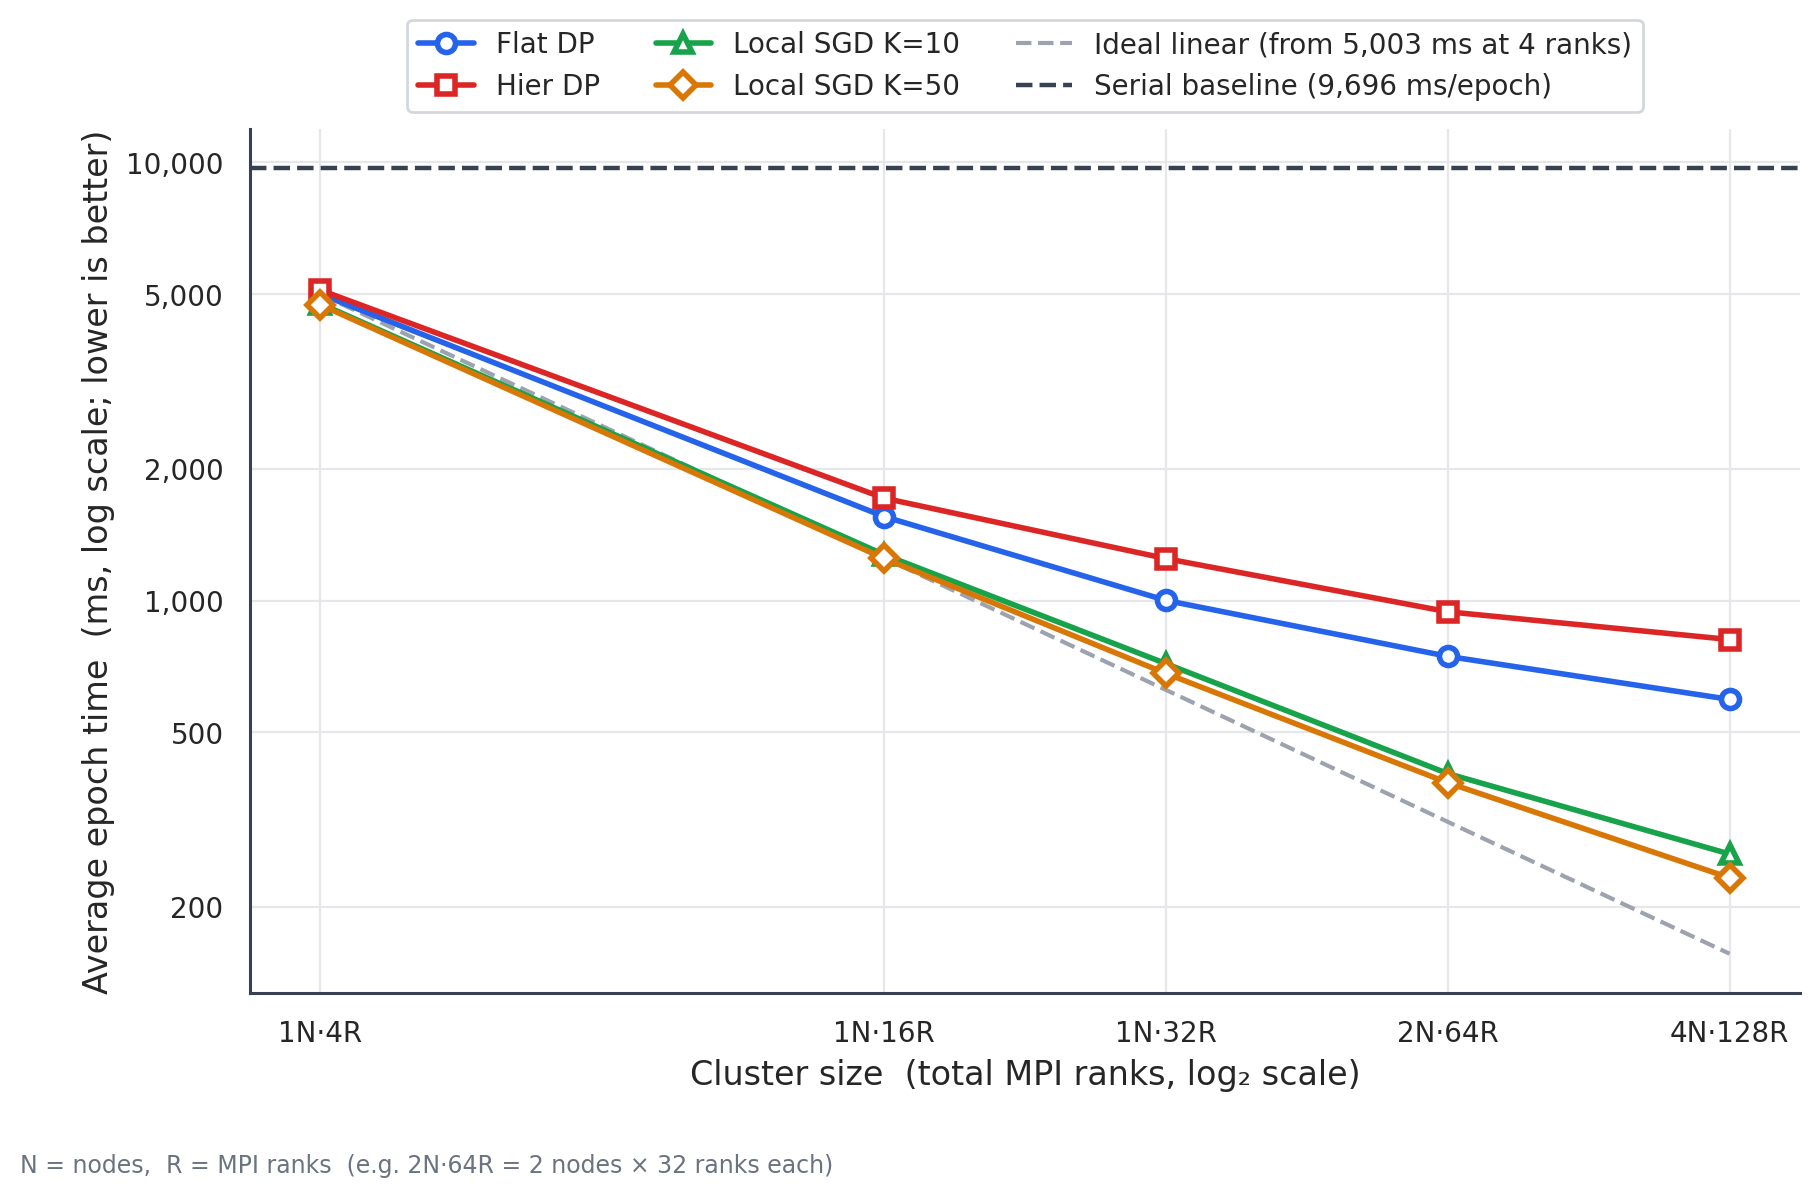
\includegraphics[width=0.88\linewidth]{images/07_time_vs_cluster_with_serial.png}
  \caption{Epoch time vs cluster size with serial baseline and ideal line
  (MLP \(256\rightarrow128\rightarrow64\), MNIST, 10 epochs).}
  \label{fig:epoch-vs-cluster}
\end{figure}

\paragraph{Strong scaling.}
Using flat DP at \(1n4r\) as baseline (\(\approx 5003\) ms/epoch), strong-scaling
speedup and efficiency are:

\begin{table}[H]
\centering
\caption{Strong scaling for flat DP (baseline: \(1n4r\)).}
\label{tab:strong}
\begin{tabular}{rrrr}
\toprule
\textbf{Config} & \textbf{Time (ms)} & \textbf{Speedup $S(p)$} & \textbf{Efficiency $E(p)$} \\
\midrule
1n4r   & 5003 & 1.00$\times$ & 100.0\% \\
1n16r  & 1555 & 3.22$\times$ & 80.4\% \\
1n32r  & 1001 & 5.00$\times$ & 62.5\% \\
2n64r  &  746 & 6.71$\times$ & 41.9\% \\
4n128r &  595 & 8.40$\times$ & 26.3\% \\
\bottomrule
\end{tabular}
\end{table}

Compared to flat DP, hierarchical DP trails at all tested scales in the
current runs, while Local-SGD surpasses flat DP speedup as \(K\) increases,
reaching \(21.46\times\) speedup at \(4n128r\) (K=50) relative to the flat-DP
4-rank baseline.

\paragraph{Weak scaling.}
This report focuses on strong scaling. A dedicated weak-scaling sweep
(proportionally increasing data size with rank count) is not yet included in
the current artifact set and is left as future work.

\paragraph{Additional DP observations.}
Timing breakdowns from logs show:
\begin{itemize}[nosep]
  \item flat DP: communication cost appears primarily in \texttt{allreduce\_ms},
        while \texttt{other\_ms} remains non-negligible at high ranks. Combined
        with better end-to-end epoch times, this is consistent with (but does
        not by itself prove) topology-aware optimization of
        \texttt{MPI\_Allreduce} by the MPI runtime; the exact per-call internal
        collective algorithm is not fully exposed in public documentation for
        the production MPI stack used on this system
        \citep{nersc-cray-mpich,nersc-perlmutter-network,hpe-intro-mpi}.
  \item hierarchical DP: cost is split into
        \texttt{intra\_reduce\_ms}, \texttt{inter\_allreduce\_ms}, and
        \texttt{intra\_bcast\_ms}, confirming additional synchronization phases.
  \item local-SGD: \texttt{sync\_ms} is much smaller than per-step DP comm cost
        because communication occurs only every \(K\) steps.
\end{itemize}
Accuracy trade-off is modest for the fastest local-SGD settings in these runs:
at 128 ranks, K=50 is fastest with a small validation-accuracy drop relative to
flat DP.

% ============================================================
%  NEW: Model Parallelism Results
%  Figures use \mpfig{filename} — adjust the \mpfig command
%  at the top of this file to point to your results directory.
% ============================================================

\subsubsection{Model-Parallel Results}
\paragraph{Epoch time and throughput vs.\ batch size.}
\label{sec:mp-batch}

Figure~\ref{fig:mp-batch-combined} shows epoch time and throughput as batch
size varies from 256 to 4096 at a fixed world size of 8 (layout
$2\!\times\!4$) for serial, sequential model parallel (\texttt{mpi-mp}), and
load-balanced pipeline parallel (\texttt{mpi-mp-pip}).
The model used for these experiments is
$784\!\rightarrow\!512\!\rightarrow\!512\!\rightarrow\!256\!\rightarrow\!256\!\rightarrow\!128\!\rightarrow\!64\!\rightarrow\!32\!\rightarrow\!10$,
chosen to have enough layers (8 weight matrices) to distribute meaningfully
across 8 ranks.

\begin{figure}[H]
  \centering
  \begin{subfigure}[b]{0.48\linewidth}
    \includegraphics[width=\linewidth]{\mpfig{chart1_epoch_time.png}}
    \caption{Epoch time vs.\ batch size.}
    \label{fig:mp-epoch-batch}
  \end{subfigure}
  \hfill
  \begin{subfigure}[b]{0.48\linewidth}
    \includegraphics[width=\linewidth]{\mpfig{chart1_throughput.png}}
    \caption{Throughput vs.\ batch size.}
    \label{fig:mp-throughput-batch}
  \end{subfigure}
  \caption{Model parallelism performance vs.\ batch size
           (MLP $512{\to}512{\to}256{\to}256{\to}128{\to}64{\to}32$,
           MNIST, 10 epochs, ws\,=\,8, layout $2\!\times\!4$).}
  \label{fig:mp-batch-combined}
\end{figure}

Several patterns are evident.
\begin{itemize}[nosep]
  \item \textbf{Both parallel modes are uniformly slower than serial.}
        Sequential model parallel runs at approximately $72$--$79$\,s/epoch
        across all batch sizes, roughly $2\times$ the serial baseline of
        $37$--$39$\,s. This is expected: in non-pipelined model parallelism the
        total step time equals the \emph{sum} of all ranks' compute plus
        inter-rank communication, so adding more ranks moves work between
        processes but does not reduce wall time for this model size.

  \item \textbf{Pipeline parallel is strongly batch-size sensitive.}
        At batch\,=\,256 pipeline epoch time is approximately $140$\,s
        (nearly $4\times$ serial) because the microbatch size is only 8 samples
        per slot, making per-message latency the dominant cost. As batch size
        grows the microbatch size grows proportionally and pipeline time falls
        sharply, reaching $\approx\!74$\,s at batch\,=\,2048 before rising
        slightly to $81$\,s at batch\,=\,4096. The modest increase at 4096 is
        consistent with the microbatch count rising from 32 to 64 at that point
        (see Section~\ref{sec:mp-mb}), which increases cumulative message
        latency.

  \item \textbf{Throughput gap is consistent.}
        Serial achieves $1{,}285$--$1{,}355$ samples/s.
        Sequential MP achieves $635$--$690$ samples/s ($\approx\!50\%$ of
        serial). Pipeline throughput rises from $355$ samples/s at
        batch\,=\,256 to $660$ samples/s at batch\,=\,2048, converging toward
        MP at larger batches.
\end{itemize}

\paragraph{Microbatch count sensitivity.}
\label{sec:mp-mb}

Figure~\ref{fig:mp-mb-combined} shows epoch time vs.\ microbatch count $M$ at
a fixed batch size of 4096 and ws\,=\,8, together with the per-category timing
breakdown for the pipeline runs.

\begin{figure}[H]
  \centering
  \begin{subfigure}[b]{0.48\linewidth}
    \includegraphics[width=\linewidth]{\mpfig{chart2_epoch_time.png}}
    \caption{Epoch time vs.\ microbatch count $M$.}
    \label{fig:mp-epoch-mb}
  \end{subfigure}
  \hfill
  \begin{subfigure}[b]{0.48\linewidth}
    \includegraphics[width=\linewidth]{\mpfig{chart2_timing_split.png}}
    \caption{Per-category timing breakdown (pipeline, mean across ranks).}
    \label{fig:mp-timing-split}
  \end{subfigure}
  \caption{Microbatch count sensitivity for pipeline parallelism
           (batch\,=\,4096, ws\,=\,8).}
  \label{fig:mp-mb-combined}
\end{figure}

The result is counterintuitive: \emph{fewer microbatches is faster}.
\begin{itemize}[nosep]
  \item At $M\!=\!8$ (microbatch size 512 rows) pipeline epoch time is
        $\approx\!39$\,s, nearly matching serial ($\approx\!37$\,s) and
        substantially outperforming sequential MP ($\approx\!72$\,s).
  \item At $M\!=\!32$ (microbatch size 128) epoch time rises to $\approx\!71$\,s,
        on par with sequential MP.
  \item At $M\!=\!64$ (microbatch size 64) epoch time is $\approx\!81$\,s,
        the slowest of the three despite having the highest theoretical pipeline
        efficiency $M/(M\!+\!P\!-\!1) = 89\%$.
\end{itemize}

The timing breakdown (Figure~\ref{fig:mp-timing-split}) explains this directly.
Forward communication wait (\texttt{fwd\_comm}) grows from $\approx\!18$\,s at
$M\!=\!8$ to $\approx\!47$\,s at $M\!=\!32$ and $\approx\!55$\,s at
$M\!=\!64$, growing roughly linearly with $M$. Each microbatch requires a
separate MPI point-to-point send across the activation boundary, so cumulative
latency accumulates as $M \cdot (\alpha + \beta m_a)$. For MNIST activations
the tensor is small (e.g.\ $512\!\times\!512$ floats at $M\!=\!8$, smaller
still at higher $M$), meaning startup cost $\alpha$ dominates over bandwidth
cost $\beta m_a$. Increasing $M$ therefore multiplies latency proportionally
without a corresponding increase in useful compute per message, overwhelming the
theoretical bubble-fraction benefit that motivates larger $M$ values.

\paragraph{Scaling with world size.}
\label{sec:mp-ws}

Figure~\ref{fig:mp-epoch-ws} shows epoch time vs.\ world size at
batch\,=\,4096 and $M\!=\!32$, with 2 tasks per node across configurations
$\mathrm{ws}\in\{2,4,6,8\}$.

\begin{figure}[H]
  \centering
  \includegraphics[width=0.78\linewidth]{\mpfig{chart4_epoch_time.png}}
  \caption{Epoch time vs.\ world size for all model-parallel modes
           (batch\,=\,4096, $M\!=\!32$, 2 tasks/node).
           Serial shown as dashed reference at $\approx\!37$\,s.}
  \label{fig:mp-epoch-ws}
\end{figure}

\begin{itemize}[nosep]
  \item \textbf{Sequential model parallel does not improve with world size.}
        Epoch time is essentially flat at $\approx\!72$--$73$\,s across all
        tested world sizes. This is the expected behavior: the non-pipelined
        schedule serializes all ranks, so adding more ranks subdivides the
        compute but adds proportional communication hops, leaving total wall
        time unchanged.

  \item \textbf{Pipeline parallel shows modest improvement with world size.}
        Unbalanced pipeline drops from $\approx\!84$\,s at ws\,=\,2 to
        $\approx\!79.5$\,s at ws\,=\,8. Load-balanced pipeline improves more
        consistently, from $\approx\!82$\,s at ws\,=\,2 to $\approx\!71.5$\,s
        at ws\,=\,8, converging toward the sequential MP baseline at the largest
        world size tested.

  \item \textbf{Serial remains faster than all parallel variants at every world size.}
        At $\approx\!37$\,s/epoch the serial baseline sits well below all
        model-parallel configurations. Throughput (Figure~\ref{fig:mp-throughput-ws})
        confirms this: serial achieves $\approx\!1{,}345$ samples/s vs.\
        $\approx\!700$ samples/s for the best parallel variant at ws\,=\,8.
\end{itemize}

\begin{figure}[H]
  \centering
  \includegraphics[width=0.78\linewidth]{\mpfig{chart4_throughput.png}}
  \caption{Throughput vs.\ world size (batch\,=\,4096, $M\!=\!32$,
           2 tasks/node).}
  \label{fig:mp-throughput-ws}
\end{figure}

\paragraph{Load-balanced layer assignment.}
\label{sec:mp-balance}

The architecture
$784\!\rightarrow\!512\!\rightarrow\!512\!\rightarrow\!256\!\rightarrow\!256\!\rightarrow\!128\!\rightarrow\!64\!\rightarrow\!32\!\rightarrow\!10$
has highly skewed layer costs: the first weight matrix
($784\!\times\!512$, $\approx\!401{,}000$ parameters) accounts for roughly
45\% of total computation, while the last three layers together account for
under 1\%. Naive round-robin assignment concentrates this imbalance on rank 0
while later ranks sit idle at each pipeline stage boundary. The load-balanced
partitioner distributes layers greedily to equalize total parameter count per
rank.

Figure~\ref{fig:mp-balance} quantifies the improvement as
$(t_{\text{pip}} - t_{\text{bal}}) / t_{\text{pip}} \times 100$, and
Table~\ref{tab:mp-balance} summarizes the values.

\begin{figure}[H]
  \centering
  \includegraphics[width=0.78\linewidth]{\mpfig{chart4_balanced_improvement.png}}
  \caption{Load-balanced pipeline improvement over naive round-robin assignment
           (batch\,=\,4096, $M\!=\!32$, 2 tasks/node).
           Positive values indicate the balanced partitioner is faster.
           Zero at ws\,=\,8 is expected: with 8 layers and 8 ranks every rank
           owns exactly one layer under both strategies.}
  \label{fig:mp-balance}
\end{figure}

\begin{table}[H]
\centering
\caption{Load-balanced pipeline improvement over naive layer assignment
         by world size (batch\,=\,4096, $M\!=\!32$, 2 tasks/node).}
\label{tab:mp-balance}
\begin{tabular}{rrrr}
\toprule
\textbf{ws} & \textbf{Unbalanced (s)} & \textbf{Balanced (s)} & \textbf{Improvement} \\
\midrule
2 & $\approx 84.0$ & $\approx 82.2$ & $+2.1\%$ \\
4 & $\approx 80.8$ & $\approx 77.5$ & $+4.1\%$ \\
6 & $\approx 79.4$ & $\approx 74.5$ & $+6.1\%$ \\
8 & $\approx 71.5$ & $\approx 71.5$ & $+0.0\%$ \\
\bottomrule
\end{tabular}
\end{table}

Improvements increase monotonically with world size up to ws\,=\,6, peaking at
$+6.1\%$. The peak at ws\,=\,6 reflects the worst-case imbalance for the naive
partitioner: 8 layers across 6 ranks forces 2 ranks to hold 2 layers each, and
naive assignment places both heavy layers on the earliest ranks. The balanced
partitioner selects which layers are grouped based on cost rather than rank
index. At ws\,=\,8 each rank holds exactly one layer under both strategies, so
the result is identical at $+0.0\%$.

\paragraph{Summary: model parallelism vs.\ serial.}
\label{sec:mp-summary}

Across all configurations tested, model parallelism does not surpass the serial
baseline for this workload. Speedup relative to serial remains at approximately
$0.5\times$ for all world sizes and both pipeline strategies
(Figure~\ref{fig:mp-speedup}), confirming that communication overhead and the
sequential nature of layer-wise activation exchange dominate over any compute
savings from distributing the model.

\begin{figure}[H]
  \centering
  \includegraphics[width=0.78\linewidth]{\mpfig{chart4_speedup.png}}
  \caption{Speedup vs.\ serial baseline for model-parallel modes
           (batch\,=\,4096, $M\!=\!32$, 2 tasks/node).
           All modes remain at $\approx\!0.5\times$, indicating that model
           parallelism at this scale imposes a net overhead relative to serial.}
  \label{fig:mp-speedup}
\end{figure}

The positive result is that the load-balanced partitioner consistently
outperforms naive round-robin when world size does not evenly divide the layer
count, and the pipeline schedule with a small microbatch count ($M\!=\!8$)
can match serial epoch time at batch\,=\,4096. The negative result is that
neither strategy overcomes the fundamental overhead of point-to-point
activation exchange at this model and hardware scale. These findings are
consistent with prior work suggesting that model parallelism is most beneficial
when individual layers are too large to fit on a single device~\citep{ref3},
a condition not met by this MNIST MLP.

% ============================================================
\section{Challenges and Obstacles}
\label{sec:challenges}
% ---------------------------------------------------------------
% Obstacles encountered.
% Hypotheses for things that did not work as expected.
% ---------------------------------------------------------------

\paragraph{[Challenge 1].} TODO: describe what you tried, what
happened, and your hypothesis for why.

\paragraph{[Challenge 2].} TODO.

\paragraph{[Challenge 3].} TODO.

% ============================================================
% Bibliography
% ============================================================
\bibliographystyle{plainnat}
\bibliography{references}   % reads references.bib

% If you prefer inline bibliography, uncomment the block below
% and remove the two lines above.
%
% \begin{thebibliography}{9}
% \bibitem{ref1}
%   Author A, Author B.
%   \textit{Title of paper 1}.
%   Venue, Year.
% \bibitem{ref2}
%   TODO
% \bibitem{ref3}
%   TODO
% \end{thebibliography}

\end{document}